\documentclass[12pt,a4paper]{article}
\usepackage[utf8]{inputenc}
\usepackage[T1]{fontenc}
\usepackage{geometry}
\geometry{a4paper, margin=1in}
\usepackage{hyperref}
\usepackage{xcolor}
\usepackage{titlesec}
\usepackage{enumitem}
\usepackage{tikz}
\usetikzlibrary{shapes.geometric, arrows.meta, positioning, fit, backgrounds, calc}
\usepackage{adjustbox}

\title{\textbf{Digital Worker Architecture: Current vs. Proposed Flow}}
\author{Architecture Review}
\date{\today}

\begin{document}

\maketitle

\section*{Executive Summary}
This document outlines the transition of the Digital Worker architecture from a proactive "Scan and Observe" model to an event-driven "Omnichannel and Caching" model. The proposed architecture significantly reduces AI processing costs and improves response times by introducing a System Memory database for reusing execution steps.

\newpage
% -----------------------------------------------------------
% CURRENT ARCHITECTURE SECTION
% -----------------------------------------------------------
\section{Current Architecture Flow}
The current system operates proactively by scanning the AWS environment based on predefined Key Result Areas (KRAs).

\subsection*{Detailed Workflow Steps}
\begin{enumerate}[label=\textbf{\arabic*.}]
    \item \textbf{User Configuration:} The user logs into the UI and defines their operational goals (KRAs).
    \item \textbf{Scan \& Observe (\textit{observationNode}):} The system wakes up and runs 11 AWS scanning tools simultaneously. It returns a detailed report (observations, issues, cost) which is displayed in the Frontend UI for the user to review.
    \item \textbf{Analysis \& Ticketing (\textit{analyzerNode}):} Once the user selects issues to pursue, the system scores their severity, calculates if \textit{humanReviewNeeded} is required, and automatically creates a new Jira ticket for each problem found.
    \item \textbf{Approval Center:} The system checks if human review is needed. If not, the action is Auto-Approved. If yes, it waits for Human Approval in the UI. Rejected or escalated actions bypass execution.
    \item \textbf{Generate Execution Steps (\textit{executionNode}):} For approved actions, the AI generates the code or Terraform commands needed to fix the problem and validates the plan.
    \item \textbf{Execution \& Resolution (\textit{action\_executor}):} The fix runs safely inside an isolated sandbox. Finally, the system closes the Jira ticket it created and saves all logs to the Audit database.
\end{enumerate}

\begin{figure}[htbp]
\centering
\begin{adjustbox}{max width=\textwidth, max height=0.75\textheight, keepaspectratio}
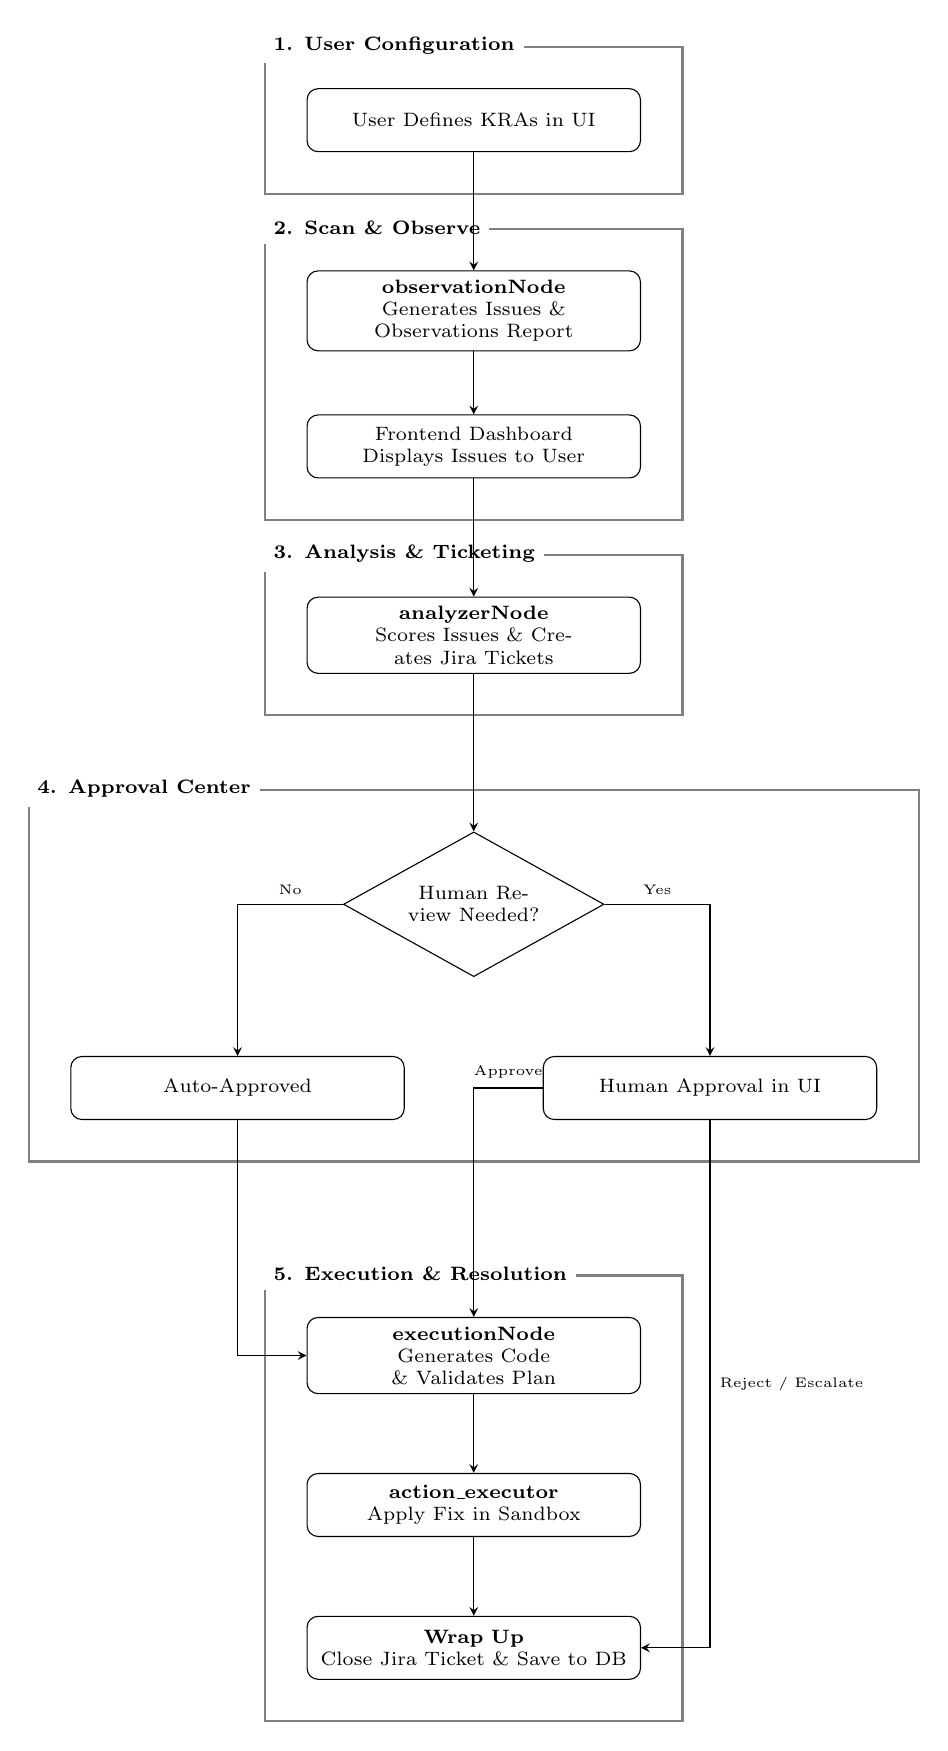
\begin{tikzpicture}[
    >=stealth,
    node distance=1cm and 1.5cm,
    box/.style={rectangle, draw, rounded corners, fill=white, text width=4cm, align=center, minimum height=0.8cm, font=\scriptsize},
    decision/.style={diamond, aspect=1.8, draw, fill=white, text width=2.5cm, align=center, inner sep=0pt, font=\scriptsize},
    groupbox/.style={rectangle, draw, inner sep=15pt, draw=gray, thick},
    grouptitle/.style={fill=white, font=\scriptsize\bfseries}
]

% 1. User Config
\node[box] (user) at (0, 0) {User Defines KRAs in UI};
\begin{scope}[on background layer]
    \node[groupbox, fit=(user)] (g1) {};
    \node[grouptitle, right] at (g1.north west) {1. User Configuration};
\end{scope}

% 2. Observe
\node[box, below=1.5cm of user] (obs) {\textbf{observationNode}\\Generates Issues \& Observations Report};
\node[box, below=0.8cm of obs] (dash) {Frontend Dashboard\\Displays Issues to User};
\begin{scope}[on background layer]
    \node[groupbox, fit=(obs) (dash)] (g2) {};
    \node[grouptitle, right] at (g2.north west) {2. Scan \& Observe};
\end{scope}

% 3. Analyze
\node[box, below=1.5cm of dash] (analyzer) {\textbf{analyzerNode}\\Scores Issues \& Creates Jira Tickets};
\begin{scope}[on background layer]
    \node[groupbox, fit=(analyzer)] (g3) {};
    \node[grouptitle, right] at (g3.north west) {3. Analysis \& Ticketing};
\end{scope}

% 4. Approval Center
\node[decision, below=2cm of analyzer] (human_rev) {Human Review Needed?};
\node[box, below=1cm of human_rev, xshift=-3cm] (auto) {Auto-Approved};
\node[box, below=1cm of human_rev, xshift=3cm] (ui_app) {Human Approval in UI};
\begin{scope}[on background layer]
    \node[groupbox, fit=(human_rev) (auto) (ui_app)] (g4) {};
    \node[grouptitle, right] at (g4.north west) {4. Approval Center};
\end{scope}

% 5. Execution Strategy & Resolution
\node[box, below=2.5cm of auto, xshift=3cm] (exec) {\textbf{executionNode}\\Generates Code \& Validates Plan};
\node[box, below=1cm of exec] (sandbox) {\textbf{action\_executor}\\Apply Fix in Sandbox};
\node[box, below=1cm of sandbox] (audit) {\textbf{Wrap Up}\\Close Jira Ticket \& Save to DB};
\begin{scope}[on background layer]
    \node[groupbox, fit=(exec) (sandbox) (audit)] (g5) {};
    \node[grouptitle, right] at (g5.north west) {5. Execution \& Resolution};
\end{scope}

\draw[->] (user) -- (obs);
\draw[->] (obs) -- (dash);
\draw[->] (dash) -- (analyzer);

\draw[->] (analyzer) -- (human_rev);
\draw[->] (human_rev) -| node[above, near start, font=\tiny] {No} (auto);
\draw[->] (human_rev) -| node[above, near start, font=\tiny] {Yes} (ui_app);

\draw[->] (auto) |- (exec);
\draw[->] (ui_app.west) -| node[above, near start, font=\tiny] {Approve} (exec.north);
\draw[->] (ui_app.south) |- node[right, near start, font=\tiny] {Reject / Escalate} (audit.east);

\draw[->] (exec) -- (sandbox);
\draw[->] (sandbox) -- (audit);

\end{tikzpicture}
\end{adjustbox}
\caption{Current Architecture Flow}
\end{figure}

\newpage
% -----------------------------------------------------------
% PROPOSED ARCHITECTURE SECTION
% -----------------------------------------------------------
\section{Proposed Architecture Flow}
The new architecture shifts to an event-driven model that listens to external channels (Jira, Slack, Teams) and introduces a "System Memory" database to bypass the AI when encountering previously solved problems.

\subsection*{Detailed Workflow Steps}
\begin{enumerate}[label=\textbf{\arabic*.}]
    \item \textbf{Request Channels:} A request arrives via Jira, Slack, or Microsoft Teams instead of a predefined KRA scan.
    \item \textbf{Intake \& Analysis:} The Digital Worker receives the request and extracts the \textit{Action Name}, \textit{Description}, and \textit{Priority Level} (P1, P2, P3).
    \item \textbf{Generate Execution Steps (The Thinking Phase):} Before asking a human for approval, the Digital Worker figures out the plan:
    \begin{itemize}
        \item \textit{Database Cache Route:} The system checks the Past History Database. If the problem is recognized, it fetches the previous Execution Steps.
        \item \textit{LLM Route:} If the problem is new, the system asks the AI Brain (Claude LLM) to generate completely new Execution Steps.
    \end{itemize}
    \item \textbf{Approval Center:} The system evaluates the Priority Level:
    \begin{itemize}
        \item \textit{Standard Priority (P2/P3):} The task is Auto-Approved by the Digital Worker and proceeds to execution.
        \item \textit{High Priority (P1):} The task requires Human Approval. A manager reviews the Action Name, Description, and the proposed Steps.
    \end{itemize}
    \item \textbf{Execution \& Resolution:} If approved, the Digital Worker performs the Execution Steps in AWS.
    \item \textbf{Wrap-Up:} The Digital Worker updates the status (Close Jira Ticket / Reply in Chat: Task Done). If the steps were newly generated by the AI, they are saved to the Past History Database for future reuse.
\end{enumerate}

\begin{figure}[htbp]
\centering
\begin{adjustbox}{max width=\textwidth, max height=0.85\textheight, keepaspectratio}
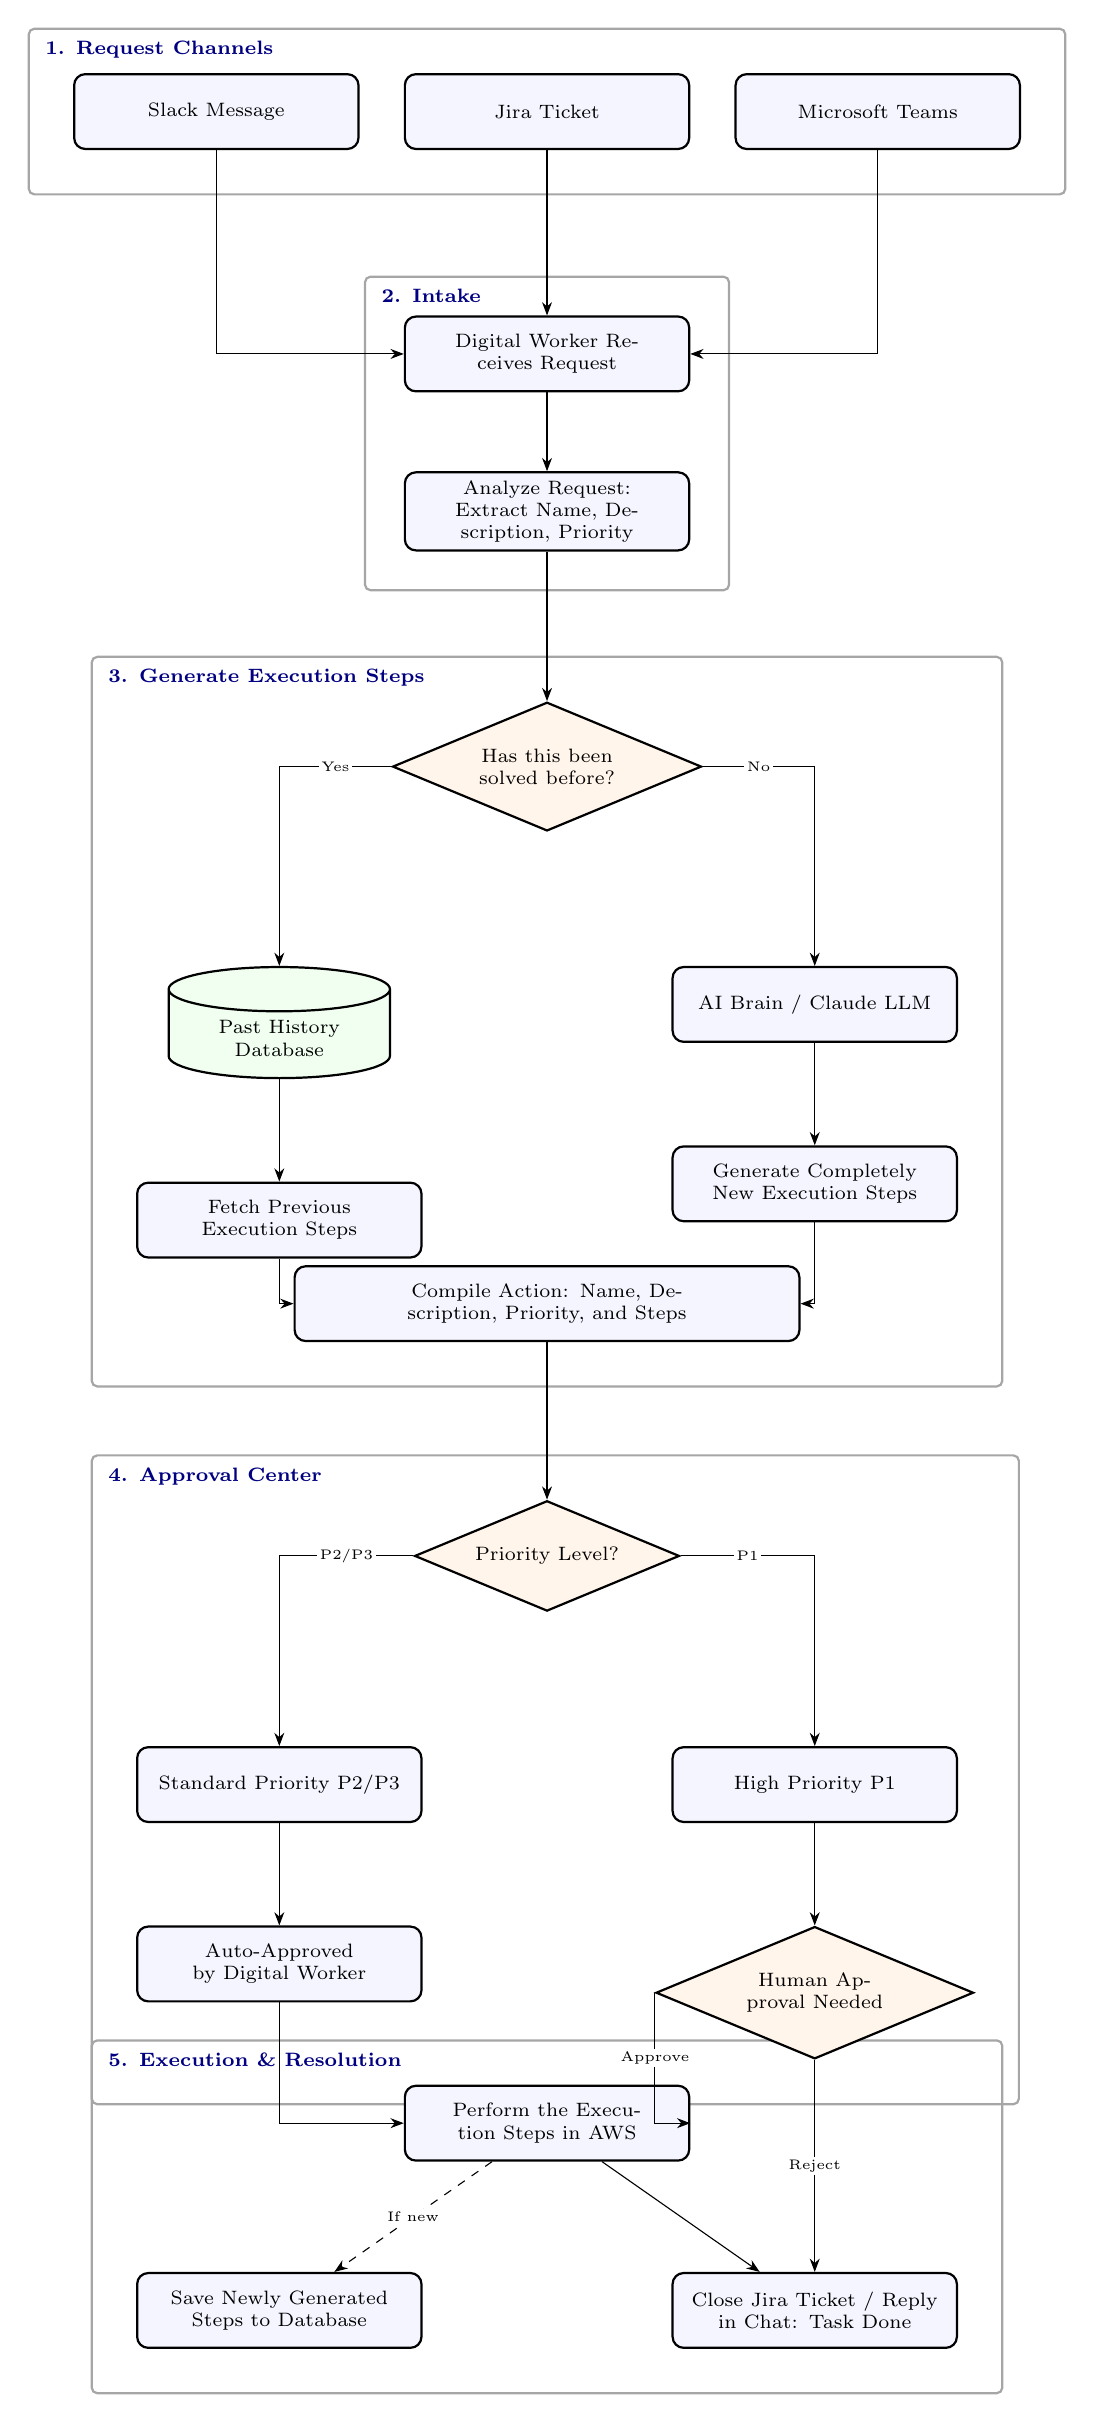
\begin{tikzpicture}[
    >=Stealth,
    every node/.style={font=\scriptsize},
    box/.style={rectangle, draw, thick, rounded corners, fill=blue!4, text width=3.4cm, align=center, minimum height=0.95cm, inner sep=3pt},
    dbbox/.style={cylinder, draw, thick, shape border rotate=90, aspect=0.2, fill=green!6, text width=2.6cm, align=center, minimum height=1.1cm, inner sep=3pt},
    decision/.style={diamond, aspect=2.4, draw, thick, fill=orange!8, text width=2.6cm, align=center, inner sep=1pt},
    groupbox/.style={rectangle, draw, gray!70, thick, inner sep=14pt, rounded corners=2pt},
    grouptitle/.style={fill=white, font=\bfseries\scriptsize, text=blue!50!black},
    lbl/.style={font=\tiny, fill=white, inner sep=1pt}
]

% ============================================================
% 1. REQUEST CHANNELS
% ============================================================
\node[box] (slack) at (-4.2, 0)  {Slack Message};
\node[box] (jira)  at (0, 0)     {Jira Ticket};
\node[box] (teams) at (4.2, 0)   {Microsoft Teams};

\begin{scope}[on background layer]
    \node[groupbox, fit=(slack)(jira)(teams), inner sep=16pt] (g1) {};
    \node[grouptitle, anchor=north west] at ($(g1.north west)+(0.1,-0.05)$) {1. Request Channels};
\end{scope}

% ============================================================
% 2. INTAKE
% ============================================================
\node[box, below=2.1cm of jira] (pickup) {Digital Worker Receives Request};
\node[box, below=1.0cm of pickup] (analyze) {Analyze Request: Extract Name, Description, Priority};

\begin{scope}[on background layer]
    \node[groupbox, fit=(pickup)(analyze), inner sep=14pt] (g2) {};
    \node[grouptitle, anchor=north west] at ($(g2.north west)+(0.1,-0.05)$) {2. Intake};
\end{scope}

\draw[->] (slack.south) |- (pickup.west);
\draw[->] (jira.south) -- (pickup.north);
\draw[->] (teams.south) |- (pickup.east);
\draw[->] (pickup) -- (analyze);

% ============================================================
% 3. GENERATE EXECUTION STEPS
% ============================================================
\node[decision, below=1.9cm of analyze] (memcheck) {Has this been solved before?};

\node[dbbox, below=1.7cm of memcheck, xshift=-3.4cm] (db) {Past History Database};
\node[box,   below=1.7cm of memcheck, xshift=3.4cm]  (ai) {AI Brain / Claude LLM};

\node[box, below=1.3cm of db] (pull)    {Fetch Previous Execution Steps};
\node[box, below=1.3cm of ai] (gennew)  {Generate Completely New Execution Steps};

% INCREASED SPACING: Placed further below memcheck to clear the branches
\node[box, below=5.5cm of memcheck, text width=6.2cm] (compile) {Compile Action: Name, Description, Priority, and Steps};

\begin{scope}[on background layer]
    \node[groupbox, fit=(memcheck)(db)(ai)(pull)(gennew)(compile), inner sep=16pt] (g3) {};
    \node[grouptitle, anchor=north west] at ($(g3.north west)+(0.1,-0.05)$) {3. Generate Execution Steps};
\end{scope}

\draw[->] (analyze) -- (memcheck);
\draw[->] (memcheck.west) -| node[lbl, pos=0.25] {Yes} (db.north);
\draw[->] (memcheck.east) -| node[lbl, pos=0.25] {No}  (ai.north);
\draw[->] (db) -- (pull);
\draw[->] (ai) -- (gennew);
\draw[->] (pull.south) |- (compile.west);
\draw[->] (gennew.south) |- (compile.east);

% ============================================================
% 4. APPROVAL CENTER
% ============================================================
\node[decision, below=2.0cm of compile] (priority) {Priority Level?};

\node[box, below=1.7cm of priority, xshift=-3.4cm] (p2p3) {Standard Priority P2/P3};
\node[box, below=1.7cm of priority, xshift=3.4cm]  (p1)   {High Priority P1};

\node[box,      below=1.3cm of p2p3] (auto)  {Auto-Approved by Digital Worker};
\node[decision, below=1.3cm of p1]   (human) {Human Approval Needed};

\begin{scope}[on background layer]
    \node[groupbox, fit=(priority)(p2p3)(p1)(auto)(human), inner sep=16pt] (g4) {};
    \node[grouptitle, anchor=north west] at ($(g4.north west)+(0.1,-0.05)$) {4. Approval Center};
\end{scope}

\draw[->] (compile) -- (priority);
\draw[->] (priority.west) -| node[lbl, pos=0.25] {P2/P3} (p2p3.north);
\draw[->] (priority.east) -| node[lbl, pos=0.25] {P1}    (p1.north);
\draw[->] (p2p3) -- (auto);
\draw[->] (p1) -- (human);

% ============================================================
% 5. EXECUTION & RESOLUTION
% ============================================================
% INCREASED SPACING: Placed further below priority to clear branches
\node[box, below=6.0cm of priority] (exec) {Perform the Execution Steps in AWS};
\node[box, below=1.4cm of exec, xshift=-3.4cm] (save)  {Save Newly Generated Steps to Database};
\node[box, below=1.4cm of exec, xshift=3.4cm]  (reply) {Close Jira Ticket / Reply in Chat: Task Done};

\begin{scope}[on background layer]
    \node[groupbox, fit=(exec)(save)(reply), inner sep=16pt] (g5) {};
    \node[grouptitle, anchor=north west] at ($(g5.north west)+(0.1,-0.05)$) {5. Execution \& Resolution};
\end{scope}

\draw[->] (auto.south) |- (exec.west);
% ROUTING FIX: Arrow exits from the west side to avoid intersection
\draw[->] (human.west) |- node[lbl, near start] {Approve} (exec.east);
% ROUTING FIX: Straight downward line since reply is directly beneath human
\draw[->] (human.south) -- node[lbl, midway] {Reject} (reply.north);
\draw[->] (exec) -- (reply);
\draw[->, dashed] (exec) -- (save) node[lbl, midway, fill=white] {If new};

\end{tikzpicture}
\end{adjustbox}
\caption{Proposed Architecture Flow}
\end{figure}

\newpage
% -----------------------------------------------------------
% BENEFITS AND CONCLUSION SECTION
% -----------------------------------------------------------
\section{Key Benefits of the Proposed Flow}
\begin{itemize}
    \item \textbf{Cost Efficiency:} By querying the System Memory first, the system entirely avoids expensive LLM calls for recurring issues.
    \item \textbf{Speed:} Fetching cached steps from PostgreSQL is nearly instantaneous compared to waiting for code generation via Claude.
    \item \textbf{Omnichannel Support:} Users can interact with the Digital Worker directly where they already work (Slack, Teams, Jira), removing the friction of a dedicated dashboard.
    \item \textbf{Safety \& Transparency:} Human managers review the exact execution steps for high-priority items \textit{before} they are approved, ensuring zero blind changes to the infrastructure.
\end{itemize}

\section{Conclusion}
The proposed event-driven architecture transforms the Digital Worker from a batch-scanning tool into a highly responsive, omnichannel AI agent. By implementing an execution memory database, the platform will become faster, cheaper to operate, and significantly more scalable as the volume of requests grows. This strategic shift perfectly aligns the Digital Worker with modern, proactive DevOps workflows.

\end{document}